
%(BEGIN_QUESTION)
% Copyright 2014, Tony R. Kuphaldt, released under the Creative Commons Attribution License (v 1.0)
% This means you may do almost anything with this work of mine, so long as you give me proper credit

Calculate $V_{AB}$ and $V_{CD}$ in this circuit, assuming both sources and transformers share a common ground and that both transformers have 1:1 winding ratios:

$$\includegraphics[width=15.5cm]{i00819x01.eps}$$

{\it Hint: since all transformers have a 1:1 turns ratio, the secondary voltage must be identical to the primary voltage for each one.  This means the phasor representing a transformer's secondary winding voltage must be exactly the same length and have exactly the same angle as the phasor representing that same transformer's primary voltage.  Treat each phasor as a line segment you are free to move around so long as you do not alter its length or direction, and you can see how they ``stack up'' onto each other according to how the windings are electrically connected to form a complete phasor diagram.}

\underbar{file i00819}
%(END_QUESTION)





%(BEGIN_ANSWER)

\noindent
{\bf Graphical (phasor diagram) solution:}

$$\includegraphics[width=15.5cm]{i00819x02.eps}$$

%(END_ANSWER)





%(BEGIN_NOTES)

\noindent
{\bf Symbolic solution:}

$$V_{AB} = V_A - V_B = (240 \hbox{ V} \angle -37^o) - (108 \hbox{ V} \angle 70^o) = 290.55 \hbox{ V} \angle -57.82^o$$

Note that due to the straight isolation of the upper transformer and the phase inversion of the lower transformer, $V_C = V_A$ and $V_D = - V_B$

$$V_{CD} = V_C - V_D$$

$$V_{CD} = V_A - (-V_B)$$

$$V_{CD} = V_A + V_B = (240 \hbox{ V} \angle -37^o) + (108 \hbox{ V} \angle 70^o) = 232.61 \hbox{ V} \angle -10.64^o $$









\vfil \eject

\noindent
{\bf Summary Quiz:}

Calculate the amount of voltage between points B and D in this circuit ($V_{BD}$), assuming both sources and transformers share a common ground and that both transformers have 1:1 winding ratios:

$$\includegraphics[width=15.5cm]{i00819x01.eps}$$

\begin{itemize}
\item{} 216.0 volts $\angle$ $70.0^o$
\vskip 5pt 
\item{} 240.0 volts $\angle$ $143^o$
\vskip 5pt 
\item{} 108.0 volts $\angle$ $-110^o$
\vskip 5pt 
\item{} 480.0 volts $\angle$ $-37.0^o$ 
\vskip 5pt 
\item{} 0.0 volts
\vskip 5pt 
\item{} 232.6 volts $\angle$ $-10.6^{o}$
\end{itemize}

%INDEX% Electronics review: AC transformer circuit
%INDEX% Electronics review, phasor expressions of circuit quantities

%(END_NOTES)


